\chapter{Background} \label{Background}

\todo*{10-15\%; thorough review of the state of the art; informed audience}


	In this chapter a general understanding of \gls{SMPC} and the key features of \glspl{MANET} is established.  
	
	First the idea for \gls{SMPC} is introduced in \ref{Secure Multi-Party Computation} \nameref{Secure Multi-Party Computation}. Since secret sharing is used for the development of \gls{SMPC} protocols, Shamir's secret sharing scheme is presented in \ref{Secret Sharing} \nameref{Secret Sharing}.
	Protocols for secure addition and secure comparison with passive security are introduced in \ref{Secure Addition Protocol} and \ref{Secure Comparison Protocol} and existing frameworks for \gls{SMPC} are briefly discussed in \ref{Existing Frameworks}.
	
	To be able to define requirements for the new framework (see \ref{Requirements}), the key features of \glspl{MANET} are identified in \fullref{Mobile Ad Hoc Networks}, with a focus on the wireless technology standards Bluetooth and Wi-Fi and the differences to similar network types like mesh networks.
	
	%Since the \gls{SMPC} protocols expect a secure communication channel, while a pairing-less connection doesn't provide security by default, public key cryptography is needed (see \ref{Securing the Communication Channel}). 
	%The key generation, as well as Shamir's secret sharing scheme, requires random numbers. Computer systems can generate pseudo-random numbers and the randomness of such an \gls{PRNG} is discussed in\fullref{Communication Layer}.
	
	\section{Secure Multi-Party Computation} \label{Secure Multi-Party Computation}
	
		\todo*{general idea}
		\gls{SMPC} is a subfield of cryptography. The target of \gls{SMPC} is to run computations over inputs from multiple parties while keeping these inputs secret. In 1982 Yao described the problem of two millionaires trying to find out, which one is wealthier, without giving each other information about their actual capital \autocite{Yao1982}. Yaos solution for this \gls{2PC} is considered to be the basis for general \gls{SMPC} protocols.
		\textcite{Cramer2015} describe for example benchmark analysis as a use-cases for \gls{SMPC}: companies want to know how well they are doing in their business area compared to other companies, while they do not want to share their current business numbers with competitors. Using a protocol for secure comparison (as described in \fullref{Secure Comparison Protocol}) the companies can calculate the best performer without leaking business information. 
		\textcite{Clifton2002} describe privacy preserving data mining as another use-case: data mining on patient data can for example be used to indicate disease outbreaks but there is of course a privacy concern. Using \gls{SMPC} algorithms, statistics can be computed while keeping the personal patient data private.
		
		For \gls{SMPC} two types of adversaries have to be considered: semi-honest and malicious adversaries.
		Semi-honest adversaries "follow the protocol specification, yet may attempt to learn additional information by analyzing the transcript of messages received during the execution" \autocite{Aumann2007}. Malicious adversaries "are not bound in any way to following the instructions of the specified protocol" \autocite{Aumann2007}.
		\gls{SMPC} protocols that can tolerate semi-honest parties (up to a specific threshold) provide semi-honest or passive security. \gls{SMPC} protocols that are secure against malicious adversaries achieve malicious or active security.
		\textcite[p. 82]{Cramer2015} also differentiate between unconditional or perfect security and computational security: if security can be proven for an adversary with unlimited computation power a protocol has unconditional security. In contrast, computational security can only be proven for a polytime adversary.
		
		Since the target group for the protocols used in this thesis are gamification systems potential adversaries are likely of the semi-honest type. Gamification system are usually based on intrinsic motivation. Especially in the context of workplace related gamification without public recognition, there is nothing to be gained from trying to corrupt the system, only the significance of the computation results is reduced.
		
		Honest, but curious parties are more likely, but providing the majority of semi-honest parties (which is the requirement for gaining additional information from combined shares, see \ref{Secret Sharing}), requires considerable efforts. Even if single scores are revealed, their isolated information content is almost valueless for the adversaries and targeting specific nodes over a longer amount of time adds additional complexity because of the spatial degree of freedom of the nodes (compare \ref{Mobile Ad Hoc Networks}).
		Therefor, in context of gamification systems, this thesis focuses on practical \gls{SMPC} protocols for passive security based on secret sharing.

		\subsection{Secret Sharing}	\label{Secret Sharing}
		
		\textcite[p. 32]{Cramer2015} describe secret sharing schemes as the main tool to build a \gls{SMPC} protocol with passive security. In 1979 Adi Shamir described a $(k, n)$ threshold scheme for sharing secret data $D$: "Our goal is to divide $D$ into $n$ pieces $D_i$, ..., $D_n$ in such a way that:
		(1) knowledge of any k or more $D_i$ pieces makes $D$ easily computable; (2) knowledge of any $k-1$ or fewer $D_i$ pieces leaves $D$ completely undetermined (in the sense that all its possible values are equally likely)" \autocite{Shamir1979}.
		Shamir's secret sharing scheme is based on polynomials of degree $k-1$ with $a_0=D$ (compare \ref{eq:polynomial}). 
		\begin{equation}
		\label{eq:polynomial}
		q(x)=\underbrace{D}_{a_0} + a_1 \cdot x + ... + a_{k-1} \cdot x^{k-1}
		\end{equation}
		
		To divide $D$ into $n$ pieces the polynomial is evaluated: $D_i=q(i),\ i=1,...,n$. For cryptographic protocols it is not practical to work with real arithmetic, instead a finite field is used: \textcite{Shamir1979} specifies that modular instead of real arithmetic is used. A prime $p$ with $p>D$, $p>n$ is selected and used to define the set $[0, p)$. "The coefficients $a_1, ..., a_{k-1}$ in $q(x)$ are randomly chosen	from a uniform distribution over the integers in $[0, p)$, and the values $D_1, ..., D_n$ are computed modulo $p$" \autocite[p. 613]{Shamir1979} (compare \ref{eq:polynomial modular}).
		\begin{equation}
		\label{eq:polynomial modular}
		q(x) = D + a_1 \cdot x + ... + a_{k-1} \cdot x^{k-1} \mod p \qquad D,\ a_i \in [0,p)\ , \quad p \in \mathbb{P}
		\end{equation}
		\textcite[p. 7]{Cramer2015} declare the set restricted by $p$ as $\mathbb{Z}_p = \{0, 1, ..., p-1\}$. They also use the notion \textit{secret S} for the data to be shared and \textit{shares $s_i$} for the computed pieces of the secret.
		
		\todo*{describe number off messages, usage of threshold as trade-off between security and performance -> START}
			
		\todo*{describe number off messages, usage of threshold as trade-off between security and performance -> END}
		
		The reconstruction of a secret $S$ can be done using Lagrange interpolation (compare \ref{eq:SSS lagrange interpolation}).
		\begin{equation}
		\label{eq:SSS lagrange interpolation}
		S = \sum_i s_i \prod_{i \neq j} \frac{-x_j}{x_i-x_j} \mod p
		\end{equation}
		 $k$ shares $s_i$ are needed to reconstruct $S$, so only the associated values for $i$ are used in the Lagrange interpolation.
						
		\subsubsection*{Example Computation} \label{Example Computation}
		
		Consider the following task: a secret $S=8$ is supposed to be shared among $n=4$ parties $P_i,\quad i=1,...,4$. The threshold for the number of needed shares for the reconstruction of the secret shall be $k=3$ (public).
		
		First a prime $p$ has to be chosen, which has to be larger than the secret ($p>S$) and the number of parties ($p>n$): $p=17$ (public information)
		
		Since $k=3$, the polynomial has a degree of $k-1=2$ (compare \ref{eq:SSS example polynomial}).
		\begin{equation}
		\label{eq:SSS example polynomial}
		f(x) = S + a_1 \cdot x + a_2 \cdot x^2 \mod p
		\end{equation}
		 
		 The coefficients are selected randomly uniformly out of $\mathbb{Z}_p=\{0,1,...,p-1\}=\{0,1,...,16\}$: $a_1=13$ and $a_2=4$ and the shares $s_i$ are computed (compare \ref{eq:SSS example polynomial specific}).
		 \begin{alignat}{1}
		 & f(x) = 8 + 13 \cdot x + 4 \cdot x^2 \mod 17 \label{eq:SSS example polynomial specific} \\
		 &\qquad \qquad \qquad \quad \Downarrow \nonumber \\ 
		 & f(x_1)=f(1)=25\mod17=8=s_1 \nonumber \\
		 & f(x_2)=f(2)=50\mod17=16=s_2 \nonumber \\
		 & f(x_3)=f(3)=83\mod17=15=s_3 \nonumber \\
		 & f(x_4)=f(4)=124\mod17=5=s_4 \nonumber 
		 \end{alignat}
		 
		 If for example parties $P_2$, $P_3$ and $P_4$ pool their shares, they can reconstruct the secret S using Lagrange interpolation (using also the public information: $p=17$):
		 \begin{alignat}{2}
		 & S = && \sum_i s_i \prod_{i \neq j} \frac{-x_j}{x_i - x_j } \mod 17 \qquad \qquad  with \ i,j \in \{2,3,4\} \\
		 & \quad && =s_2 \cdot \frac{-x_3}{x_2-x_3} \cdot \frac{-x_4}{x_2-x_4} + s_3 \cdot \frac{-x_2}{x_3-x_2} \cdot \frac{-x_4}{x_3-x_4} + s_4 \cdot \frac{-x_2}{x_4-x_2} \cdot \frac{-x_3}{x_4-x_3} \mod 17 \nonumber \\
		 & \quad && =16 \cdot \frac{-3}{2-3} \cdot \frac{-4}{2-4} + 15 \cdot \frac{-2}{3-2} \cdot \frac{-4}{3-4} + 5 \cdot \frac{-2}{4-2} \cdot \frac{-3}{4-3} \mod 17  \nonumber \\
		 & \quad && = 96-120+15 \mod 17 \nonumber \\
		 & \quad && = -9 \mod 17 \label{eq:SSS example negative modulo} \\
		 & \quad && = 8 \nonumber 
		 \end{alignat}
		 \textit{Note:} in cryptography $a \mod n$ for $a<0$ (negative dividend) is calculated by adding a multiple of  $n$ ($mn\mod n=0$), so that $m \cdot n+a>0$: e.g. $-9 \mod 17 = (\underbrace{1 \cdot 17-9}_{>0}) \mod 17$ (compare \ref{eq:SSS example negative modulo}), which resolves to: $a\mod n = n-(|a|\mod n), a<0$.
		 
		%\subsection*{Differential Privacy}
		\todo*{Write about differential privacy?}
		
		\subsection{Secure Addition Protocol} \label{Secure Addition Protocol}
		
		For an environment with honest parties there are simple \gls{SMPC} protocols to compute the sum over shares. \textcite{Clifton2002} describe a ring based method, where the initializing party adds a random number $R$ to the secret input $s_1$ before passing it to the next node. Each node then adds its secret until the first party receives the result. By removing $R$ the party can than reconstruct the sum over all secret inputs (see figure \ref{figure:smpc sum ring}).
		
		\begin{figure}[!htb] % h for placement here
		\caption{Simple secure sum protocol for ring} \label{figure:smpc sum ring}
		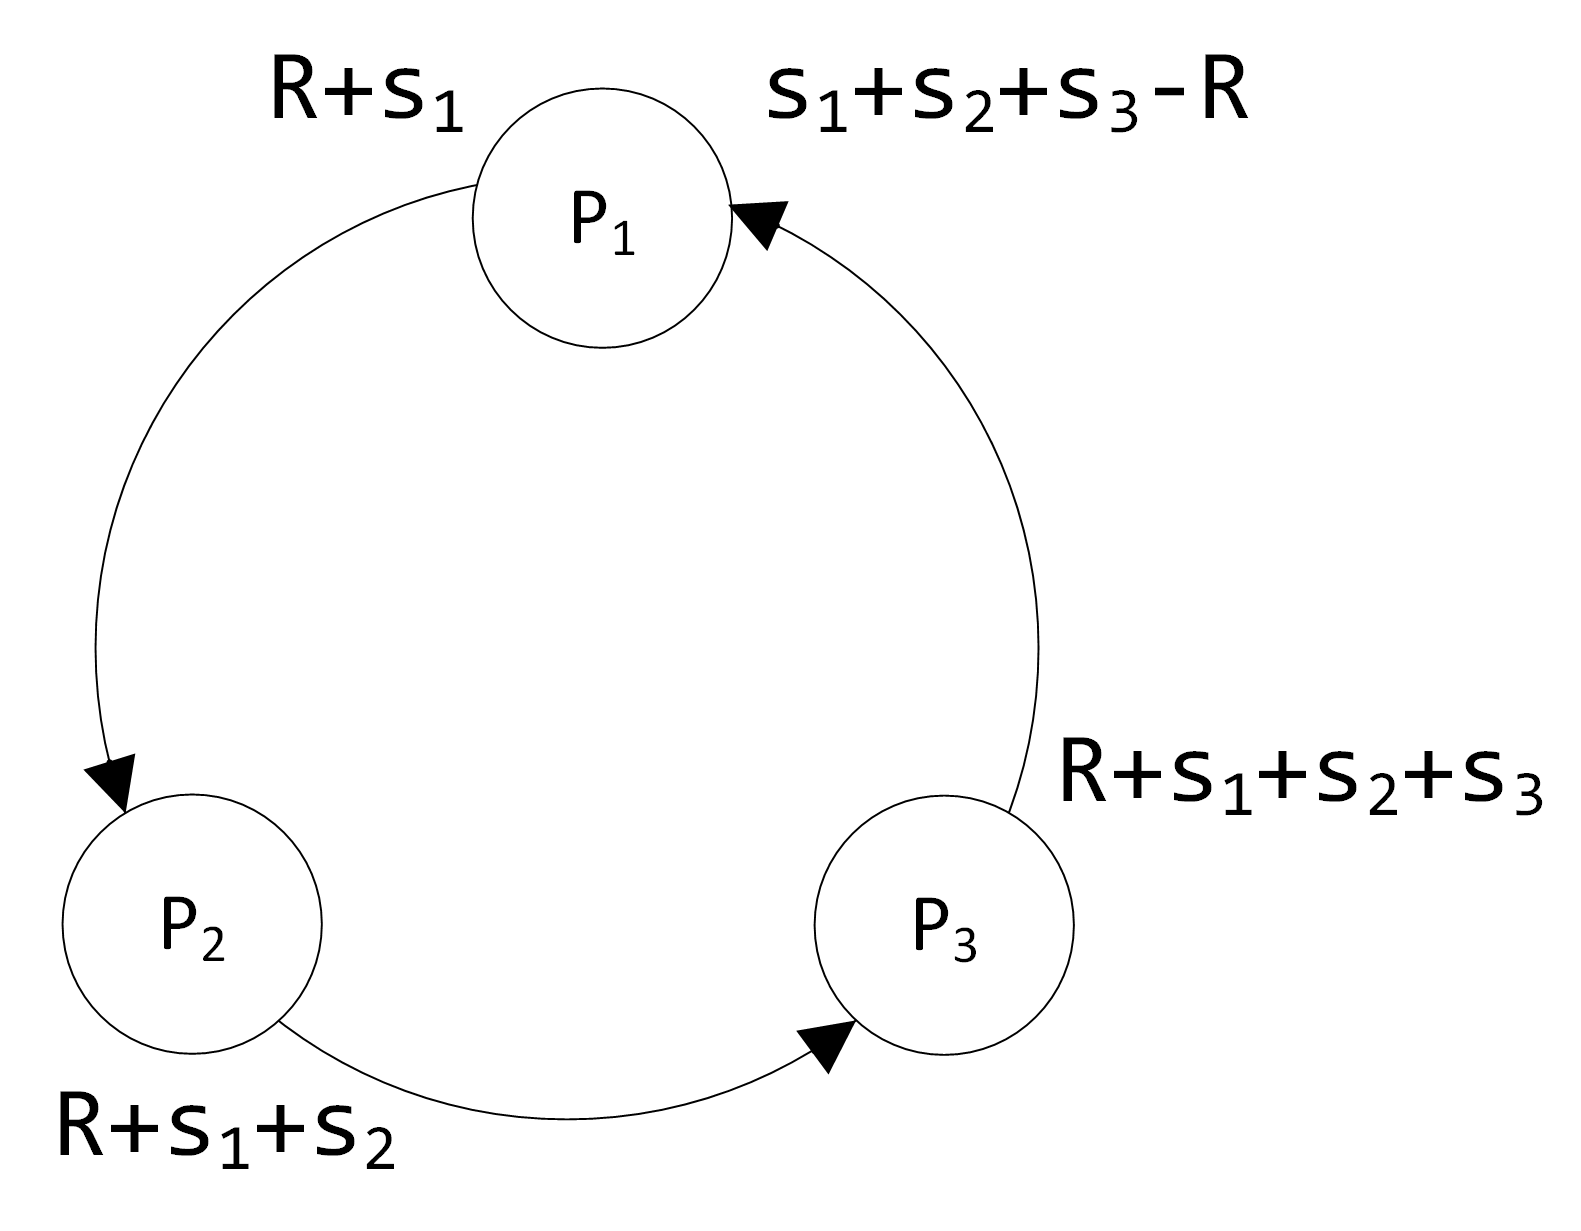
\includegraphics[scale=1.0]{figures/smpc-sum-simple-ring.png}
		\end{figure}
		
		This method is efficient ($2n$ messages for computation and announcing the sum in a $n$-node ring) but if parties collude, party $P_i$ only needs the output of $P_{i+1}$ as received by party $P_{i+2}$ to reconstruct the secret input of $P_{i+1}$. \textcite{Clifton2002} propose using shares in combination with permutation of the ring order, so neighbors change in each iteration and the number of parties in need to pool their data increases. This approach was extended in the "k-Secure Sum Protocol" \autocite{Sheikh2009}. Especially with a focus on security ($k\rightarrow n$) the permutation of the ring approaches share-exchanges between each node. To reduce the complexity through the ring permutation and motivated by the restrictions of the network (see \ref{Implementability}), for which the protocol is intended, this thesis  uses a Shamir based protocol for a fully connected mesh network. 
		
		In \ref{Secret Sharing} it was demonstrated how a secret can be reconstructed from the shares using Lagrange interpolation. It is also possible to reconstruct the sum of secrets by using the sums of shares for a Lagrange interpolation.
		
		Proof:
		
		$n$ shares for $m$ secrets $s_l$:
		\begin{alignat}{1}
			&s_{l,i} = f_l(x_i) = s_l + \sum_{i=1}^{k-1} \alpha_{l,i} x_i^i \mod p \\
			& \Leftrightarrow \begin{cases}
				s_{1,i} = f_1(x_i) = & s_1 + \alpha_{1,1} x_i + \alpha_{1,2} x_i^2 + ... + \alpha_{1,k-1}x_i^{k-1} \mod p \\
				&\vdots \\
				s_{m,i} = f_n(x_i) = & s_n + \beta_{n,1} x_i + \beta_{n,2} x_i^2 + ... + \beta_{n,k-1}x_i^{k-1} \mod p
			  \end{cases} \nonumber \\
			& \text{with} \ \{l \in \mathbb{N} \ | \ 1 \leq l \leq m \},
			\ \{i \in \mathbb{N} \ | \ 1 \leq i \leq n \},
			\ \{ p \in \mathbb{P} \ | \ p > \sum_l s_l \}, \nonumber \\
			&\{ \alpha \in \mathbb{N} \ | \ 0 \leq \alpha \leq p \},
			\ \{k \in \mathbb{N} \ | \ 2 < k \leq n \} \nonumber
		\end{alignat}
		
		Lagrange-interpolation for secret $s_l$:
		\begin{alignat}{1}
			&s_l = \sum_{i=1}^{n}s_{l,i}\prod_{i\neq j}\frac{-x_j}{x_i - x_j} \mod p \label{eq:Lagrange for s_l}
		\end{alignat}
		Sum $s$ over secrets $s_l$:
		\begin{alignat}{1}
			&s = \sum_{l=1}^{m} s_l \overset{\text{with} \ \ref{eq:Lagrange for s_l}}{=} \sum_{l=1}^{m} \sum_{i=1}^{n} s_{l,i}\prod_{i\neq j} \frac{-x_j}{x_i-x_j} \mod p \label{eq:sum over secrets}
		\end{alignat}
		\begin{alignat}{1}
		&\text{with} \quad \sum_{i=1}^{n}\sum_{j=1}^{m}a_{ij} = \sum_{j=1}^{m}\sum_{i=1}^{n}a_{ij} \quad \text{follows for \ref{eq:sum over secrets}} \nonumber\\
		&s= \underbrace{ \sum_{i=1}^n \underbrace{\sum_{l=1}^{m} s_{l,i}}_{\text{sum over shares}} \prod_{i\neq j} \frac{-x_j}{x_i-x_j} \mod p }_{\text{Lagrange-interpolation for sum over shares}}
		\end{alignat}	
		
		\subsubsection*{Example Computation}
		Public information: $n=4$, $p=67$, $k=4$\par
		
		\noindent Secrets: $s_1=13$, $s_2=27$, $s_3=17$, $s_4=1$\par
		
		\noindent Target computation: sum $s$ over secrets $s= \sum_{i=1}^4 s_i=58$ without revealing ones secret to another party.		
		\begin{alignat}{1}
			s_{1,i}&=f_1(x_i)=13 + 35x + 22x^2 + 7x^3 \mod 67 \label{eq:example shares 1,i} \\
			s_{2,i}&=f_2(x_i)=27 + 3x + 19x^2 \mod 67 \label{eq:example shares 2,i} \\
			s_{3,i}&=f_3(x_i)=17 + 9x^2 + 27x^3 \mod 67 \label{eq:example shares 3,i} \\
			s_{4,i}&=f_4(x_i)=1 + 13x + 31x^2 + 40x^3 \mod 67 \label{eq:example shares 4,i}
		\end{alignat}
		with $x_1=1$, $x_2=2$, $x_3=3$, $x_4=4$ follows
		\begin{alignat}{7}
		 \overset{\ref{eq:example shares 1,i}}{\Rightarrow} s_{1,1}&=10 \quad &&s_{1,2}&&=26 \quad &&s_{1,3}&&=36 \quad  &&s_{1,4}&&=15  \nonumber \\
		\overset{\ref{eq:example shares 2,i}}{\Rightarrow} s_{2,1}&=49 \quad &&s_{2,2}&&=42 \quad &&s_{2,3}&&=6 \quad &&s_{2,4}&&=8  \nonumber \\
		\overset{\ref{eq:example shares 3,i}}{\Rightarrow} s_{3,1}&=53 \quad &&s_{3,2}&&=1 \quad &&s_{3,3}&&=23 \quad &&s_{3,4}&&=13  \nonumber \\
		\overset{\ref{eq:example shares 4,i}}{\Rightarrow} s_{4,1}&=18 \quad &&s_{4,2}&&=2 \quad &&s_{4,3}&&=59 \quad &&s_{4,4}&&=27 \nonumber \\
		\Rightarrow \sum_l s_{l,1}&=130 \quad \sum_l && s_{l,2}&&=71 \quad \sum_l && s_{l,3}&&=124 \quad \sum_l && s_{l,4}&&=63 \nonumber		
		\end{alignat}
		Lagrange-interpolation:
		\begin{alignat}{2}
		s&= &&\sum_{i=1}^{4}\sum_{l=1}^{4}s_{l,i}\prod_{i \neq j} \frac{-x_j}{x_i-x_j}\mod 67 \nonumber \\
		 &= &&130\frac{-2}{1-2}\frac{-3}{1-3}\frac{-4}{1-4}+71\frac{-1}{2-1}\frac{-3}{2-3}\frac{-4}{2-4} \nonumber \\
		 & &&+124\frac{-1}{3-1}\frac{-2}{3-2}\frac{-4}{3-4}+63\frac{-1}{4-1}\frac{-2}{4-2}\frac{-3}{4-3}\mod 67 \nonumber \\
		 &=&& 527 \mod 67 = 58 = \sum_{i=1}^4 s_i \label{eq:example result lagrange}
		\end{alignat}
		As expected, the result of the Lagrange-interpolation for the sum over shares is equal to the sum over the initial secrets (compare \ref{eq:example result lagrange}).
		
		\subsubsection*{Protocol Description}
		Assumptions:
		%\vspace{-\topsep}
		\begin{itemize}
			%\itemsep-0.5em
			\item number of parties $n>2$
			\item secure communication channel
			\item no malicious adversaries
			\item upper bound of sum $s \leq b$ can be estimated, so a prime $p > b$ can be chosen 
		\end{itemize}
		The secure addition protocol, as used in this thesis, consists of six phases:
		\begin{enumerate}
		%\itemsep-0.5em
		\item The coordinator announces the number of parties for the computation and the indexation of each party.
		\item Each party $j$ sends shares $s_{j,i}$ of the secret input $s_j$ to the other parties.
		\item Each party $i$ computes the sum over the received shares $s_{j,i}$.
		\item Each party sends the computed sum to the coordinator.
		\item The coordinator reconstructs the sum over the inputs using Lagrange-interpolation.
		\item The coordinator broadcasts the reconstructed sum.
		\end{enumerate}
	
		In total $(n+3)\cdot (n-1)=n^2+2n-3$ messages are exchanged, so the traffic increases with the number of parties squared. Selecting a lower threshold for the secret reconstruction $\frac{n}{2} \leq k<n$ lowers the total messages by $\Delta_{\text{messages}}=n^2-n(k-1)$.
		
		For a secure channel this protocol is information-theoretically secure: independent from computation power an adversary with $m_\text{leaked}<k$ shares will gain no information regarding the inputs.
	
		\todo*{secure addition with verification \autocite{Cramer2015}; number of messages}
		
		\subsection{Secure Comparison Protocol}	\label{Secure Comparison Protocol}
		The secure comparison protocol compares the secret inputs and provides the minimum or maximum in a set without revealing the inputs or the parties holding the minimum or the maximum.
		
		The protocol is based on the privacy preserving protocol for maximum computation as described in \textcite{Hasan2013}. The general idea is to use bit-decomposition and utilize the secure addition protocol bit-wise. In iterations the secure-sum for the bits ($0 \lor 1$) of the secrets multiplied with a random value are computed, starting from the \gls{MSB}, limited by a predefined upper bound, to the \gls{LSB}. The announced sum gives each party the information that at least one party has this bit set, if the sum is unequal zero. If a party has this bit not set itself it has a lower value and commits only zeros in the following iterations. Storing the result of each iteration, the parties can reconstruct the maximum.
		For finding the minimum the protocol from \textcite{Hasan2013} needs an extension as described in \ref{Protocol Extension for Minimum Determination}: inputs are negated (using the binary operation NOT), making the minimum in the set the largest value. Afterwards the maximum is determined as described above. Finally the found maximum is negated again to reconstruct the minimum in the set.
		
		\subsubsection{Example Computation} \label{Secure Comparison Example}
		
		Public information: $n=3$, $p=67$, $\mathbb{Z}_p=\{1,...,p-1\}$, $k=3$, $s_i<b=64$ (upper bound for secret value range) \par
		\noindent Secrets: $s_1=13$, $s_2=27$, $s_3=17$ \par
		
		\noindent Target computation: $\min(s_i)=13$, $\max(s_i)=27$
		
		Since $64_{10}=1000000_2$ is defined as upper bound for the secret values the \gls{MSB} is the sixth bit (second column in table \ref{table:secure maximum binary representation of secrets}).
		 
		\begin{table}[!htb]
			\centering
			\caption{Binary representation of secrets $s_i$} \label{table:secure maximum binary representation of secrets}
			\begin{tabular}{|c|l|l|l|l|l|l|}
				\hline
				Decimal $s_{i,10}$ & \multicolumn{6}{l|}{Binary $s_{i,2}$} \\ \hline
				13                 & 0    & 0    & 1    & 1    & 0   & 1   \\ \hline
				27                 & 0    & 1    & 1    & 0    & 1   & 1   \\ \hline
				17                 & 0    & 1    & 0    & 0    & 0   & 1   \\ \hline
			\end{tabular}
		\end{table}

		Each party multiplies each bit with a random within $\mathbb{Z_p}$:
		
		\begin{table}[!htb]
			\centering
			\caption{Randomized binary representation of secrets} \label{table:secure maximum randomized binary representation}
			\begin{tabular}{|c|l|l|l|l|l|l|l|l|l|l|l|l|}
				\hline
				Decimal $s_{i,10}$ & \multicolumn{6}{l|}{Binary $s_{i,2}$}  & \multicolumn{6}{l|}{Randomized} \\ \hline
				13                 & 0    & 0    & 1    & 1    & 0   & 1 & 0    & 0    & 45    & 61    & 0   & 57   \\ \hline
				27                 & 0    & 1    & 1    & 0    & 1   & 1 & 0    & 12    & 31    & 0    & 5   & 15   \\ \hline
				17                 & 0    & 1    & 0    & 0    & 0   & 1 & 0    & 24    & 0    & 0    & 0   & 9   \\ \hline
			\end{tabular}
		\end{table}
				
		\begin{alignat}{3}
			\intertext{There are six bits, therefore six rounds of secure addition ($\sum_{secure}$) are computed:}
			1^{st} \ \text{round:} \quad & \sum_{secure}=0 && \Rightarrow \quad 6^{th} \ \text{bit of the maximum is} && 0 \nonumber \\
			2^{nd} \ \text{round:} \quad &\sum_{secure}=36 > 0 \quad && \Rightarrow \quad 5^{th} \ \text{bit of the maximum is} \quad && 1 \nonumber \\
			\intertext{Party $p_1$ disqualifies itself as the maximum (see table \ref{table:secure maximum p1 not maximum})}
			3^{rd} \ \text{round:} \quad &\sum_{secure}=31 > 0 && \Rightarrow \quad 4^{th} \ \text{bit of the maximum is} && 1 \nonumber \\
			\intertext{Party $p_3$ disqualifies itself as the maximum (see table \ref{table:secure maximum p3 not maximum})}
			4^{th} \ \text{round:} \quad &\sum_{secure}=0 && \Rightarrow \quad 3^{rd} \ \text{bit of the maximum is} && 0 \nonumber \\
			5^{th} \ \text{round:} \quad &\sum_{secure}=5>0 && \Rightarrow \quad 2^{nd} \ \text{bit of the maximum is} && 1 \nonumber \\
			6^{th} \ \text{round:} \quad &\sum_{secure}=15>0 && \Rightarrow \quad 1^{st} \ \text{bit of the maximum is} && 1 \nonumber
		\end{alignat}

		\begin{table}[!htb]
			\centering
			\caption{$2^{nd}$ round} \label{table:secure maximum p1 not maximum}
			\begin{tabular}{|l|l|l|l|l|l|l|}
				\hline
				Decimal $s_{i,10}$ & \multicolumn{6}{l|}{Randomized} \\ \hline
				13                 & 0    & \underline{0}    & $\cancelto{0}{45}$    & $\cancelto{0}{61}$    & 0   & $\cancelto{0}{57}$   \\ \hline
				27                 & 0    & 12    & 31    & 0    & 5   & 15   \\ \hline
				17                 & 0    & 24    & 0    & 0    & 0   & 9   \\ \hline
			\end{tabular}
		\end{table}

		\begin{table}[!htb]
			\centering
			\caption{$3^{rd}$ round} \label{table:secure maximum p3 not maximum}
			\begin{tabular}{|l|l|l|l|l|l|l|}
				\hline
				Decimal $s_{i,10}$ & \multicolumn{6}{l|}{Randomized} \\ \hline
				13                 & 0    & 0    & 0    & 0    & 0   & 0   \\ \hline
				27                 & 0    & 12    & 31    & 0    & 5   & 15   \\ \hline
				17                 & 0    & 24    & \underline{0}    & 0    & 0   & $\cancelto{0}{9}$   \\ \hline
			\end{tabular}
		\end{table}

		In total, each party has the bits $0|1|1|0|1|1$ stored and can reconstruct the correct maximum $\max(s_i)=27$.
		
		\subsubsection{Protocol Extension for Minimum Determination} \label{Protocol Extension for Minimum Determination}
		
		Using the negation of the binary representation, the order of the corresponding values in decimal numeral system is inverted (compare table \ref{table:secure minimum negation}). The computation is then the same as for the maximum search. The reconstructed maximum is finally negated to result in $\min(s_i)$.
		
		\begin{table}[!htb]
			\centering
			\caption{Negation of binary representation for minimum determination} \label{table:secure minimum negation}
			\begin{tabular}{|l|l|l|l|l|l|l|l|l|l|l|l|l|}
				\hline
				Decimal $s_{i,10}$ & \multicolumn{6}{l|}{Binary $s_{i,2}$}  & \multicolumn{6}{l|}{Negated $\bar{s}_{i,2}$} \\ \hline
				13                 & 0    & 0    & 1    & 1    & 0   & 1 & 1    & 1    & 0    & 0    & 1   & 0   \\ \hline
				27                 & 0    & 1    & 1    & 0    & 1   & 1 & 1    & 0    & 0    & 1    & 0   & 0   \\ \hline
				17                 & 0    & 1    & 0    & 0    & 0   & 1 & 1    & 0    & 1    & 1    & 1   & 0   \\ \hline
			\end{tabular}
		\end{table}
	
		In the second round booth $P_2$ and $P_3$ disqualify themselves as maximum. After six rounds each party holds: $1|1|0|0|1|0$ as the maximum. Negated this gives the minimum as $0|0|1|1|0|1_2=13_{10}$ 

		\FloatBarrier
		
		\subsubsection{Protocol Description}
		Assumptions:
		% \vspace{-\topsep}
		\begin{itemize}
			% \itemsep-0.5em
			\item number of parties $n>2$
			\item secure communication channel
			\item no malicious adversaries
			\item upper bound of sum $s \leq b$ can be estimated, so a prime $p > b$ can be chosen 
		\end{itemize}
		The secure comparison protocol, as used in this thesis, consists of the phases for secure addition within iterations for the bitwise length of a predefined upper bound for the inputs: 
		\begin{enumerate}
			% \itemsep-0.5em
			\item The coordinator announces the number of parties for the computation and the indexation of each party.
			\item For minimum-search: each party negates the secret input.
			\item For each bit in the secret input starting from \gls{MSB} to \gls{LSB} each party runs through iterations:
			%\vspace{-\topsep}
			\begin{enumerate}
				% \itemsep-0.5em
				\item If input is flagged as lower than maximum, then use $s_j=0$ as the input. Otherwise multiply actual bit $b$ with a random value $R$: $s_j=b \cdot R$.
				\item Each party $j$ sends shares $s_{j,i}$ of the input $s_j$ to the other parties.
				\item Each party $i$ computes the sum over the received shares $s_{j,i}$.
				\item Each party sends the computed sum to the coordinator.
				\item The coordinator reconstructs the sum over the inputs using Lagrange-interpolation.
				\item The coordinator broadcasts the reconstructed sum.
				\item Each party stores if the sum for the bit was equal 0 (set bit 0) or unequal 0 (set bit 1).
				\item Each party compares if bit from the computed sum is greater than own bit. If so input is flagged as lower than maximum.
			\end{enumerate}
			\item For minimum-search: each party negates the stored sum-result.
		\end{enumerate}
	
		Note: the assumption $n>2$ for the secure addition and secure comparison protocols is not strict enough, if sum, $\min$ and $\max$ are computed for the same parties, since for $n=3$ the secret between minimum and maximum can be restored (for a honest majority the mapping of values to parties is still secure though).
		
		\subsection{Existing Frameworks} \label{Existing Frameworks}
		
		In this section a short overview over existing \gls{SMPC} solutions is given. While \gls{SMPC} is an intensely researched field, practical work is less common.
		
		The following solutions were considered
		
		\begin{itemize}
			\item MpcLib (see \textcite{Online:MpcLib})
			\item SEPIA (see \textcite{Online:Sepia})
			\item SPDZ (see \textcite{Online:SPDZ})
			\item Sharemind (see \textcite{Online:Sharemind})
			\item Enigma (see \textcite{Online:Enigma})
		\end{itemize}
		
		Some key-features of the solutions are illustrated in figure \ref{figure:existing frameworks}. All projects emerged from university research. With the exception of Sharemind and Enigma, the frameworks seem to target primarily other researchers, reflecting in the lack of documentation and thereby reduced usability. The open-source library MpcLib is C\# based, SPDZ uses C++ and Python and SEPIA is a Java library.  Sharemind and Enigma are also booth based on university research (Enigma at MIT and Sharemind at University of Tartu) but evolved into market-ready business solutions. While Sharemind uses dedicated application-server, Enigma uses a distributed system of nodes based on Blockchain technology for \gls{SMPC}, booth with a focus on scalable secure data analysis.
		All solution are based on the Internet protocol suite and require at least locally run server or Internet access.
		
		\begin{figure}[!htb] % h for placement here
			\caption{Existing \gls{SMPC} software grouped by properties} \label{figure:existing frameworks}
			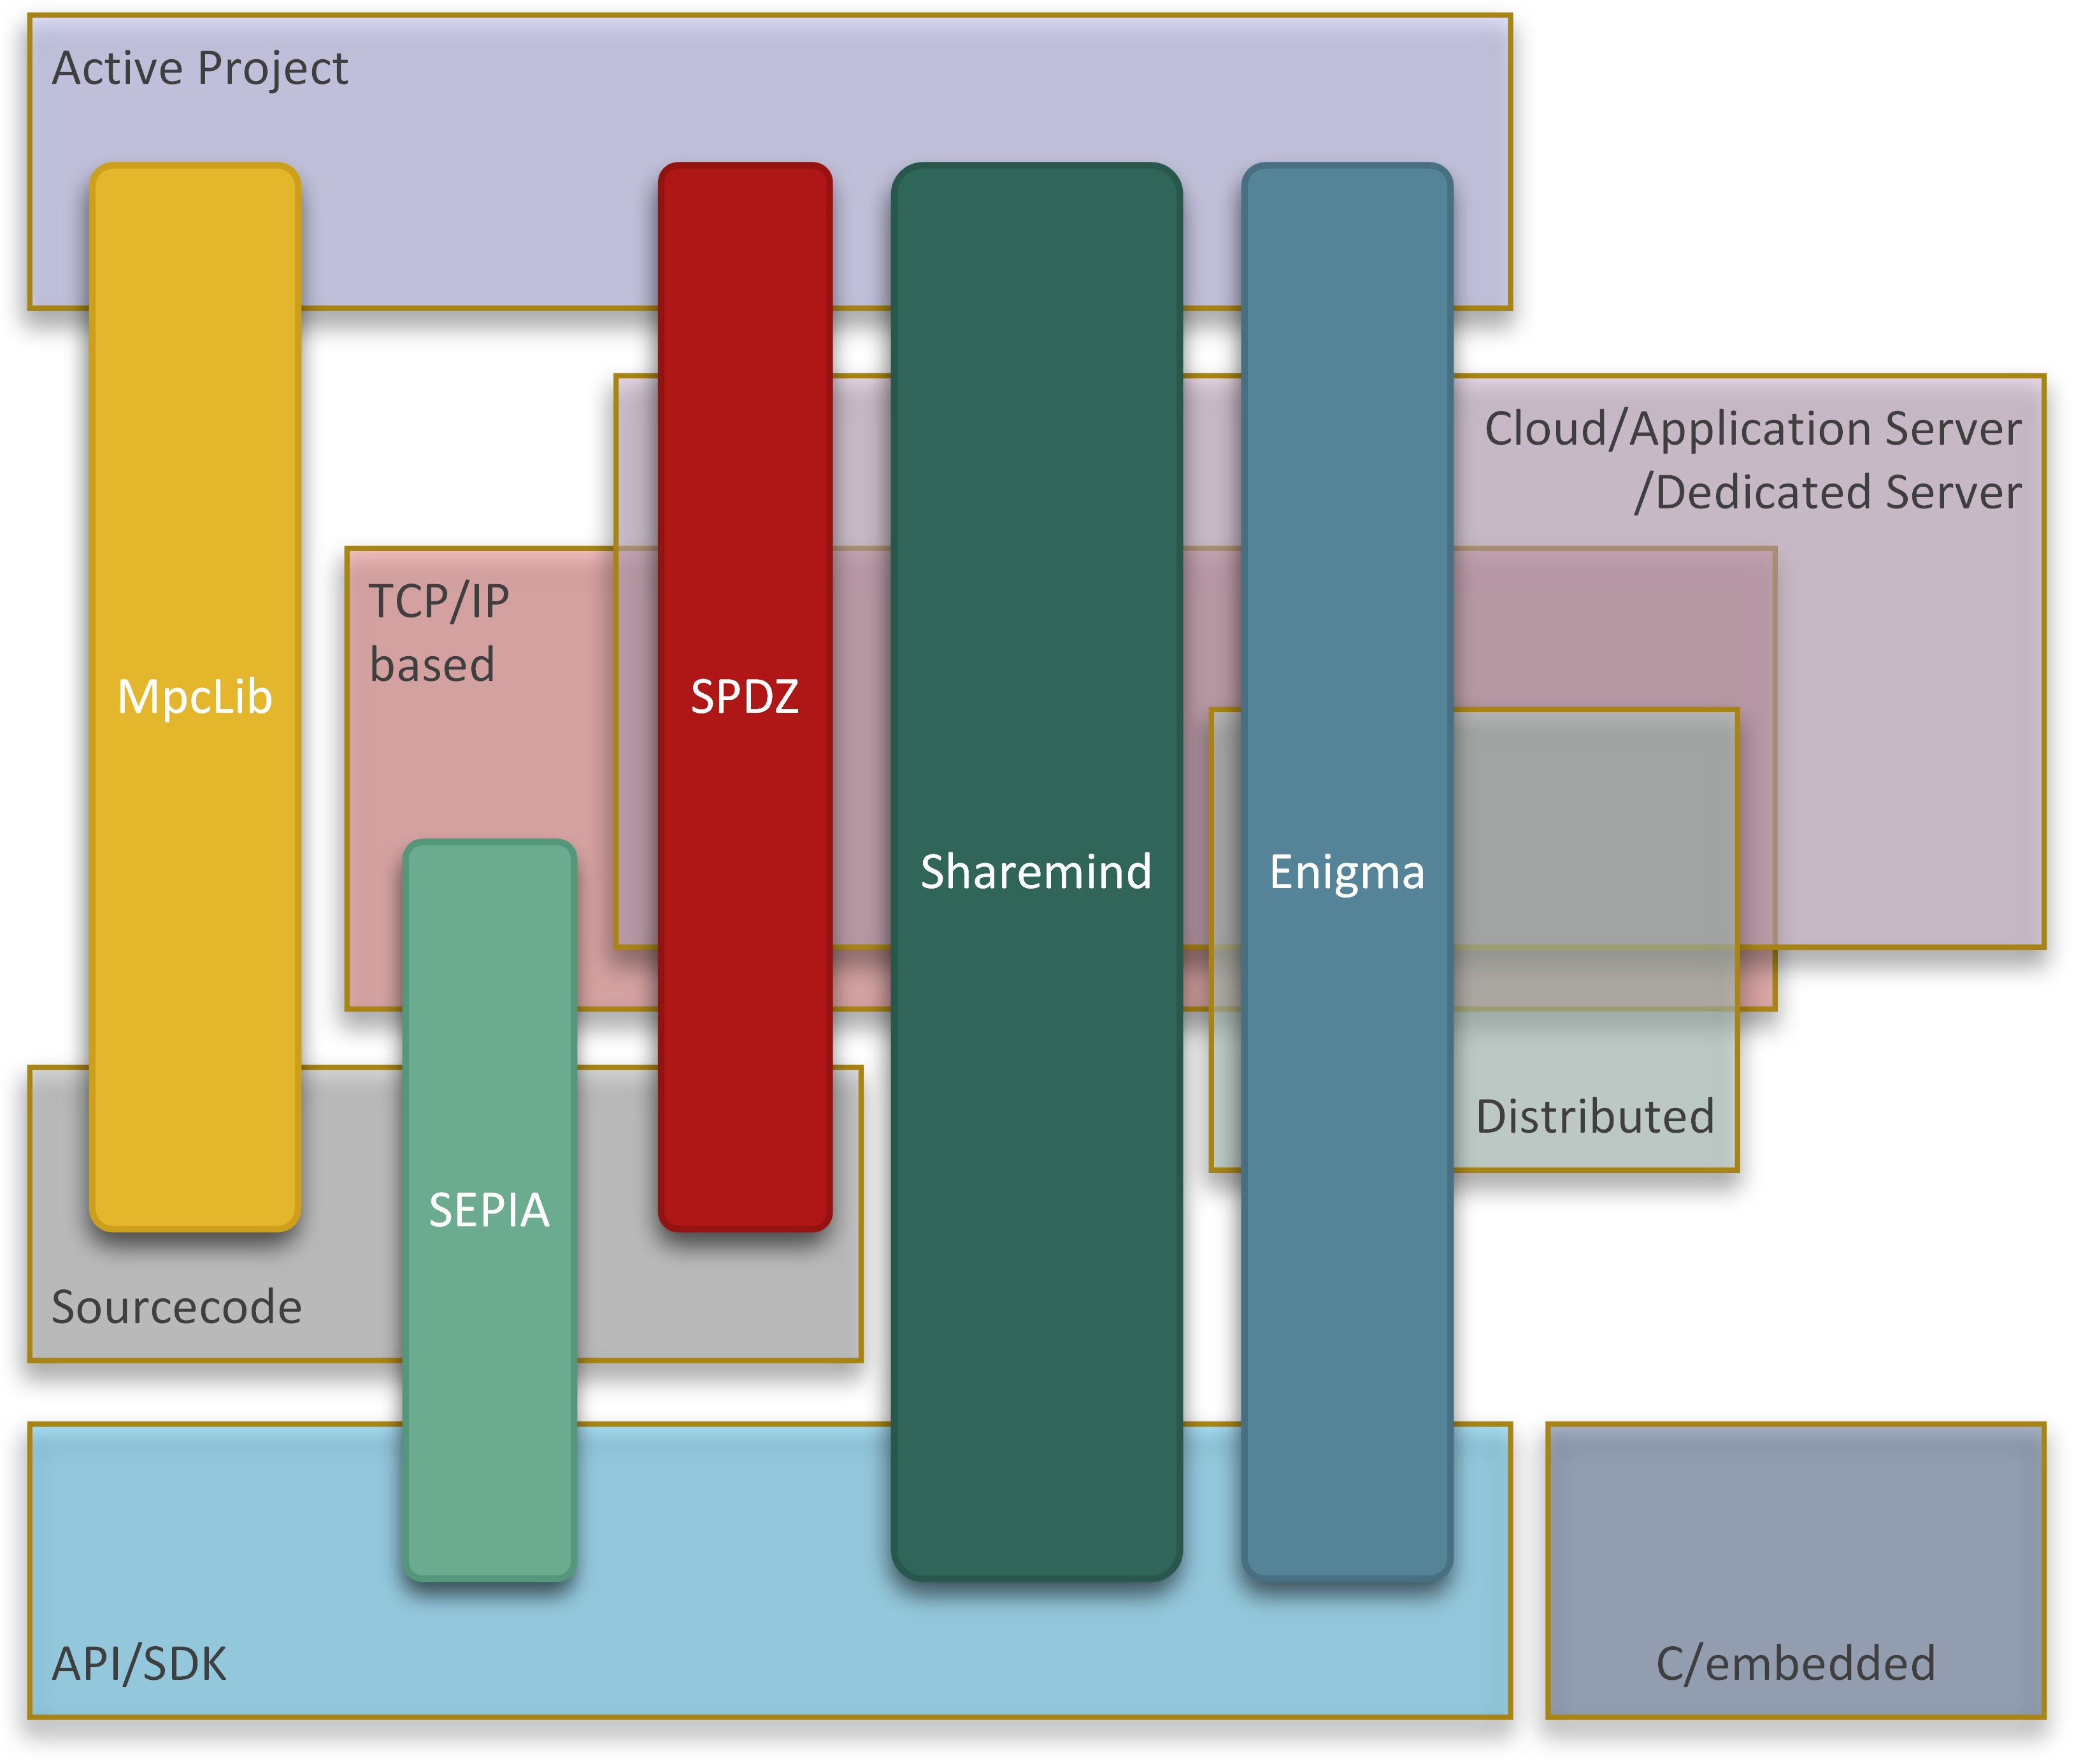
\includegraphics[scale=1.0]{figures/frameworks.png}
		\end{figure}
	
		While all frameworks exceed the requirements regarding the \gls{SMPC} functionality, they don't provide a solution for local ad-hoc networks without permanently available servers. Also the support for low-level devices is either undocumented or not given through programming language dependencies.
		The development of a framework with a focus on cross-platform usage, usability for developers without cryptographic research background and applicability for local ad-hoc networks for the described gamification use-cases is therefor justified.
		
	\FloatBarrier
	
	\section{Mobile Ad Hoc Networks}
	\label{Mobile Ad Hoc Networks}
	The framework developed as part of this thesis focuses on providing \gls{SMPC} for \glspl{MANET} or \gls{MANET}-like networks. In this section the network topologies related to \glspl{MANET} are briefly described (see \ref{Network Topologies}) and the implementability based on current technology standards are examined (see \ref{Implementability}).
		
	\subsection{Network Topologies}
	\label{Network Topologies}
	
	\textcite{Dorri2015} describe a \gls{MANET} as an "infrastructure-independent network with wireless mobile nodes" \autocite[p. 15]{Dorri2015}. \glspl{MANET} are similar to mesh networks, but the distinctive feature is the nodes' spatial degree of freedom. In comparison to a star network, there is no central switch dedicated to routing messages. Instead each node provides message passing abilities and acts as a multi-hop relay.
	The advantage of \glspl{MANET} is the open network boundary: nodes can freely join and leaving nodes do not affect the functionality of the \gls{MANET}. The key-features are:
	
	%\vspace{-\topsep}
	\begin{itemize}  
		%\itemsep-0.5em
		\item continuously self-configuring
		\item self-forming
		\item self-healing
		\item infrastructure-less
		\item peer-to-peer
		\item  mobility of nodes (main difference to mesh network)
	\end{itemize}
			
	The message passing in a \gls{MANET} can either be done by routing or flooding. Since the nodes can move freely, the neighbors will change often, so maintaining routing tables is expensive. The passing of messages without the availability of authentication protocols like \gls{HTTPS} makes the communication also vulnerable against man-in-the-middle attacks. Of course flooding means broadcasting and is not cheap either in regard to message quantity and network load.
	
	The mentioned key-features of \glspl{MANET} make it a good network choice for a gamification setting based on mobile devices (smartphones, wearables, etc.), because it promises unobtrusive usage for participants without administrative maintenance effort. In the next section the availability and the implementability for Android devices is discussed, because of Androids dominant position as the globally leading smartphone \gls{OS} with a market share of above 80\% (see \textcite{Online:Gartner2016}). 
	
	\subsection{Implementability on Android Devices} \label{Implementability}
	
	\glspl{MANET} are especially of interest for military applications and disaster management but they are also gaining research focus for civil usage for example in context of \gls{IoT} devices. Demonstrations of the implementability can be found for example in Open Gardens MeshKit \gls{SDK} \autocite{Online:MeshKit}, which offers \gls{MANET} abilities for Android and iOS devices and thereby forming a \gls{SPAN}. MeshKit is also the foundation for Open Gardens FireChat \autocite{Online:FireChat}, which is for example known in context of pro-democracy demonstrations. Since Android does not provide an \gls{API} for \gls{MANET} functionality on Android devices (\gls{API} 24 at the time of writing) and the MeshKit \gls{SDK} is not open source and only available through Open Gardens partner program, a simplified (but extendable) implementation of \gls{MANET}-like behavior is developed in the application layer (compare \ref{Coordinator Election}).
	Both for Wi-Fi and Bluetooth based connections, there can be limitations in regard to maximum concurrent connections. Vendor specific restrictions (hardware, driver) are hard to compensate reactive at runtime, so this issue has to be addressed proactive in \ref{Architecture} \nameref{Architecture}.
	
	\subsubsection{Bluetooth Based \gls{MANET}}
	
	Usually Bluetooth connections with smartphones require pairing and user actions. This is not a useful process flow to build a \gls{MANET}-like network, since nodes cannot simply join.
	Using the Bluetooth protocol \gls{RFCOMM} an insecure connection can be established, without the need for pairing and user interaction. \textcite{RFCOMM2012} describe \gls{RFCOMM} as the emulation of serial ports over \gls{L2CAP}, supporting the emulation of multiple ports between two devices and ports between multiple devices (device dependent).
	Since multiple simultaneous connection have to share the available bandwidth per node, it takes $\frac{n}{2}$ times longer to share the same amount of data when using only one-to-one connections sequentially. For the targeted number of computation partners in this thesis, this is a tolerable overhead and practical system parameters will be evaluated in \ref{Evaluation} and \ref{Discussion}.
	The Bluetooth Special Interest Group has announced mesh networking protocols for upcoming specifications \autocite{Online:BluetoothMesh}. This is very promising in regard of system provided \gls{MANET} features, though it will take time (from experience with Bluetooth LE likely years) until enough devices are equipped with compliant Bluetooth modules.

	\subsubsection{Wi-Fi Based \gls{MANET}}
			
	Situations in which we can use Wi-Fi (or \gls{GSM}) usually provide Internet access, so Wi-Fi is not the primary target technology for this thesis. Generally, the callback-based architecture of the developed framework (compare \ref{Architecture} \nameref{Architecture}) enables the usage of different wireless technologies though. Even the interconnection of \gls{MANET}-like networks is conceivable (as demonstrated with MeshKit), but it complicates the forming of the computation group (compare \ref{Coordinator Election}), because different optional channels between nodes have to be evaluated.
	With Android 4.0 (\gls{API} level 14) the Wi-Fi Peer-to-Peer framework was introduced, which complies with the Wi-Fi Alliance's Wi-Fi Direct certificate program. Wi-Fi Direct states that one-to-one or group (many-to-one) connections are possible. One device acts as a group owner (soft access point), so it forms a star topology. To imitate a \gls{SPAN} with Wi-Fi Direct multi-group communication has to be provided. In \textcite{Funai2015} limitations of Android in regard of multi-group networking as well as solutions are discussed.
	Other solutions (compare \textcite{Online:SPANProject}) include usage of custom kernels on rooted smartphones. Even though  demonstrations on selected devices have shown the feasibility, such system modifications neglect the target group and the intentions of this framework.
								
		%\section{Pseudo-Random Numbers} %maybe move to implementation/secureing channel
		%\label{sec:Pseudo-Random Numbers}
			
		%\todo*{random numbers important for cryptography: selection of coefficients in secret sharing, public key generation, ...; RNG in different environments; entropy}
			
		%https://en.wikipedia.org/wiki/Cryptographically_secure_pseudo-random_number_generator
			
		%\todo*{lib will require a callback for random number generator -> maybe mention with outlook for requirements}

\FloatBarrier